\documentclass[letterpaper, 12pt]{article}
\usepackage[utf8]{inputenc}
\usepackage[spanish]{babel}
\usepackage{amsmath, amssymb}
\usepackage{geometry}
\usepackage{fancyhdr}
\usepackage{enumitem}
\usepackage{graphicx}
\usepackage{hyperref}
\usepackage{multicol}
\usepackage{parskip}
\usepackage{xcolor}
\usepackage{tcolorbox}
\usepackage{eso-pic}
\usepackage{tikz}
\usetikzlibrary{patterns, calc, arrows.meta, positioning}
\tcbuselibrary{skins}

\geometry{letterpaper, margin=1.5cm, top=3cm, bottom=2.5cm, headheight=2cm}
\definecolor{celesteSuave}{HTML}{F0F7FF}
\definecolor{azulFuerte}{HTML}{1A5276}
\definecolor{turquesaUsach}{HTML}{33CCCC}
\definecolor{enlace}{HTML}{1A5276}
\definecolor{grisRuta}{HTML}{666666}

\newcommand{\logoup}{./images/logo_up.png}
\newcommand{\logousach}{./images/logo_usach.png}
\newcommand{\logofondo}{./images/logo_up.png}
\newcommand{\institucion}{Usach Premium}
\newcommand{\curso}{Física I para Ingeniería}
\newcommand{\guiasnumero}{Guía Práctica - Movimiento Rectilíneo Uniforme}
\newcommand{\semestre}{1er. Semestre de 2026}
\newcommand{\preparadopor}{Usach Premium}
\newcommand{\webinstitucion}{www.usachpremium.cl}
\newcommand{\instagraminstitucion}{https://www.instagram.com/usach.premium}
\newcommand{\transparencia}{0.05}
\newcommand{\fraseportada}{"Por y para estudiantes"}
\newcommand{\listacontenidos}{
    \item[\color{azulFuerte}$\Rightarrow$] Ecuación horaria del MRU.
    \item[\color{azulFuerte}$\Rightarrow$] Conversión de unidades y rapidez constante.
    \item[\color{azulFuerte}$\Rightarrow$] Encuentros, alcances y movimiento relativo.
    \item[\color{azulFuerte}$\Rightarrow$] Lectura de gráficos posición-tiempo.
}

\hypersetup{colorlinks=true, linkcolor=enlace, urlcolor=enlace, citecolor=enlace, pdfborder={0 0 0}}
\pagestyle{fancy}
\fancyhf{}
\fancyhead[L]{\includegraphics[height=1.2cm]{\logoup}}
\fancyhead[R]{%
    \begin{minipage}[b]{0.42\textwidth}
        \raggedleft\fontsize{9pt}{11pt}\selectfont
        \textbf{\color{azulFuerte}\institucion}\\
        \curso\ --- \guiasnumero\\
        \textit{\color{gray}@usach.premium}
    \end{minipage}\hspace{0.1cm}\includegraphics[height=1.2cm]{\logousach}}
\fancyfoot[L]{\fontsize{9pt}{11pt}\selectfont \textit{\fraseportada}}
\fancyfoot[R]{\fontsize{9pt}{11pt}\selectfont Página \thepage}
\renewcommand{\headrulewidth}{0.4pt}
\renewcommand{\footrulewidth}{0.4pt}
\fancypagestyle{plain}{\fancyhf{}\renewcommand{\headrulewidth}{0pt}\renewcommand{\footrulewidth}{0pt}}

\newcommand{\MarcaAgua}{
    \AddToShipoutPicture{\AtPageCenter{\makebox(0,0){%
        \begin{tikzpicture}
            \node[opacity=\transparencia, inner sep=0pt]{\includegraphics[width=0.7\textwidth]{\logofondo}};
        \end{tikzpicture}}}}
}
\newenvironment{kitpropiedades}[1]{\begin{tcolorbox}[colback=celesteSuave, colframe=azulFuerte,title=\textbf{#1}, fonttitle=\bfseries]}{\end{tcolorbox}}
\newtcolorbox{desafiobox}[1]{colback=white,colframe=azulFuerte,fonttitle=\bfseries,coltitle=white,title=#1,arc=8pt,boxrule=1.2pt,enhanced,drop shadow={black!5}}
\newenvironment{solbox}[1]{\begin{tcolorbox}[colback=celesteSuave, colframe=azulFuerte,title=\textbf{#1}, fonttitle=\bfseries]}{\end{tcolorbox}}
\newenvironment{introduccion}{\section*{Introducción}\MarcaAgua}{}
\newenvironment{ejercicios}{\MarcaAgua}{}
\newenvironment{soluciones}{%
    \newpage
    \begin{center}\begin{tcolorbox}[colback=azulFuerte, colframe=azulFuerte,colupper=white, width=0.8\textwidth, center, arc=10pt]
    \centering\Large\textbf{SOLUCIONARIO}
    \end{tcolorbox}\end{center}
    \MarcaAgua\small}{}
\tikzset{
    ruta/.style={azulFuerte, line width=1.1pt, -{Latex[length=3mm]}},
    marca/.style={circle, fill=azulFuerte, inner sep=1.8pt},
    etiqueta/.style={font=\scriptsize, align=center},
    objeto/.style={draw=azulFuerte, fill=celesteSuave, rounded corners=2pt, line width=0.8pt},
    eje/.style={-{Latex[length=2.6mm]}, grisRuta, line width=0.8pt}
}

\begin{document}
\thispagestyle{plain}
\AddToShipoutPicture*{\put(54,700){\includegraphics[width=2cm]{\logoup}}\put(420,706){\includegraphics[width=5cm]{\logousach}}}
\vspace*{0.5cm}
\begin{center}
    \color{azulFuerte}
    {\huge\textbf{GUÍA DE EJERCICIOS}}\\[0.5cm]
    {\Huge\textbf{\curso}}\\[0.3cm]
    {\Large\guiasnumero}\\[1.5cm]
    \begin{tcolorbox}[colback=celesteSuave, colframe=azulFuerte, arc=10pt,width=0.85\textwidth, center, boxrule=1.5pt]
        \centering\vspace{0.2cm}{\Large\textbf{Contenidos}}\vspace{0.3cm}
        \color{black}\begin{itemize}[leftmargin=3cm]\listacontenidos\end{itemize}\vspace{0.2cm}
    \end{tcolorbox}
\end{center}
\vspace{1.5cm}
\begin{center}{\Large\textbf{\semestre}}\\[0.8cm]{\large\textbf{\preparadopor}}\end{center}
\vspace{2cm}
\begin{center}
    {\color{azulFuerte}\hrule height 0.5pt}\vspace{0.3cm}
    \begin{minipage}{0.45\textwidth}\centering\textbf{Instagram:}\\\small\href{\instagraminstitucion}{@usach.premium}\end{minipage}
    \begin{minipage}{0.45\textwidth}\centering\textbf{Web:}\\\small\href{http://\webinstitucion}{\webinstitucion}\end{minipage}
\end{center}
\pagenumbering{arabic}
\newpage

\begin{kitpropiedades}{RESUMEN DE CLASES: LO QUE DEBES SABER}
\begin{multicols}{2}
\textbf{1. Ecuación horaria}
\begin{itemize}[leftmargin=10pt]
    \item $x(t)=x_0+vt$
    \item $\Delta x=x_f-x_i$
    \item $v=\dfrac{\Delta x}{\Delta t}$
\end{itemize}
\columnbreak
\textbf{2. Lectura física}
\begin{itemize}[leftmargin=10pt]
    \item Si $v>0$, avanza en el sentido positivo.
    \item Si $v<0$, avanza en el sentido negativo.
    \item En un gráfico $x$ vs. $t$, la pendiente es la velocidad.
\end{itemize}
\end{multicols}
\textbf{3. Conversión útil}
\begin{itemize}[leftmargin=10pt, itemsep=0.1cm]
    \item $1\,\mathrm{km}=1000\,\mathrm{m}$, \quad $1\,\mathrm{h}=3600\,\mathrm{s}$.
    \item Para pasar de $\mathrm{km/h}$ a $\mathrm{m/s}$, divide por $3{,}6$.
    \item En MRU no se usa aceleración: la rapidez permanece constante.
\end{itemize}
\begin{center}\small\textbf{Tip Pro:} Antes de reemplazar datos, dibuja el eje, marca el origen y revisa si los móviles van en sentidos opuestos.\end{center}
\end{kitpropiedades}

\begin{ejercicios}
\section*{Entrenamiento MRU}
\begin{enumerate}[label=\textbf{\arabic*.}, leftmargin=*, itemsep=0.8cm]
\item \textbf{Llegada al campus.} Un bus de acercamiento de Usach Premium avanza por una recta con rapidez constante de $54\,\mathrm{km/h}$. Usachín lo espera a $1{,}20\,\mathrm{km}$ del punto donde el bus inicia el registro de tiempo.
\begin{enumerate}[label=\alph*)]
    \item Determina el tiempo que tarda en llegar hasta Usachín.
    \item Determina la distancia recorrida durante los primeros $35\,\mathrm{s}$.
\end{enumerate}
\begin{center}
    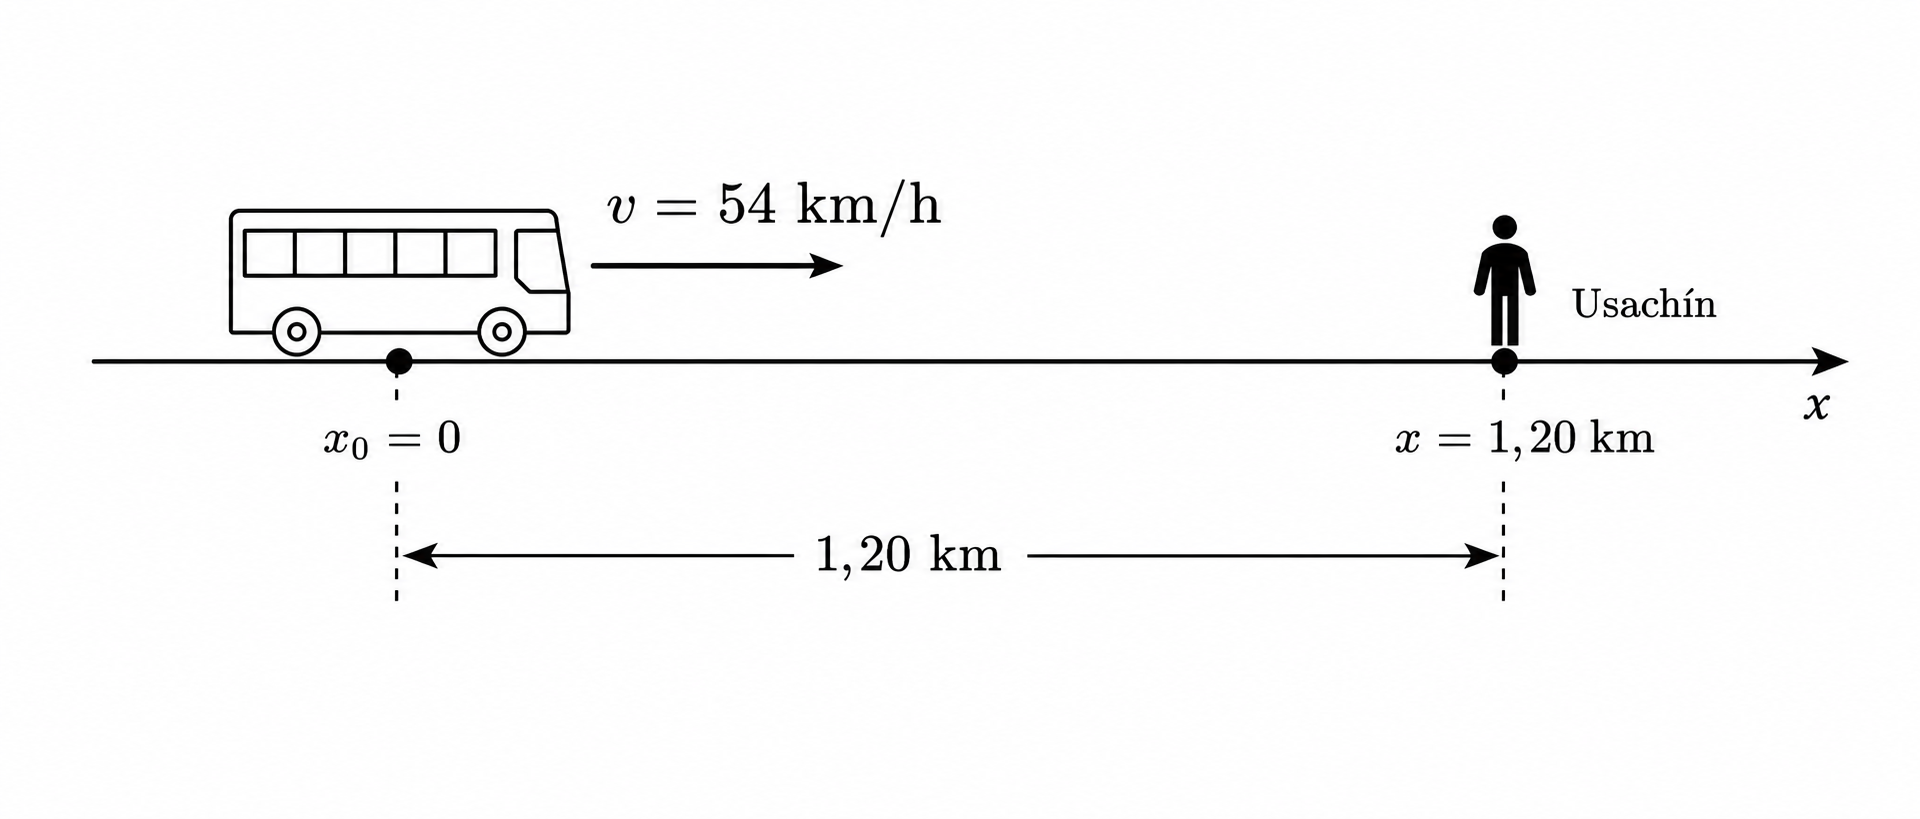
\includegraphics[width=0.86\textwidth]{./images/ejercicio1_mru.png}
\end{center}

\item \textbf{Encuentro camino al Aula Magna.} Una monitora sale desde PAIEP hacia el Aula Magna con rapidez constante $1{,}60\,\mathrm{m/s}$. La distancia entre ambos puntos se modela como una recta de $480\,\mathrm{m}$. Un segundo monitor sale desde el Aula Magna hacia PAIEP $60\,\mathrm{s}$ después, con rapidez constante $1{,}20\,\mathrm{m/s}$.
\begin{enumerate}[label=\alph*)]
    \item Determina el instante de encuentro medido desde que sale la primera monitora.
    \item Determina la posición del encuentro medida desde PAIEP.
\end{enumerate}
\begin{center}
    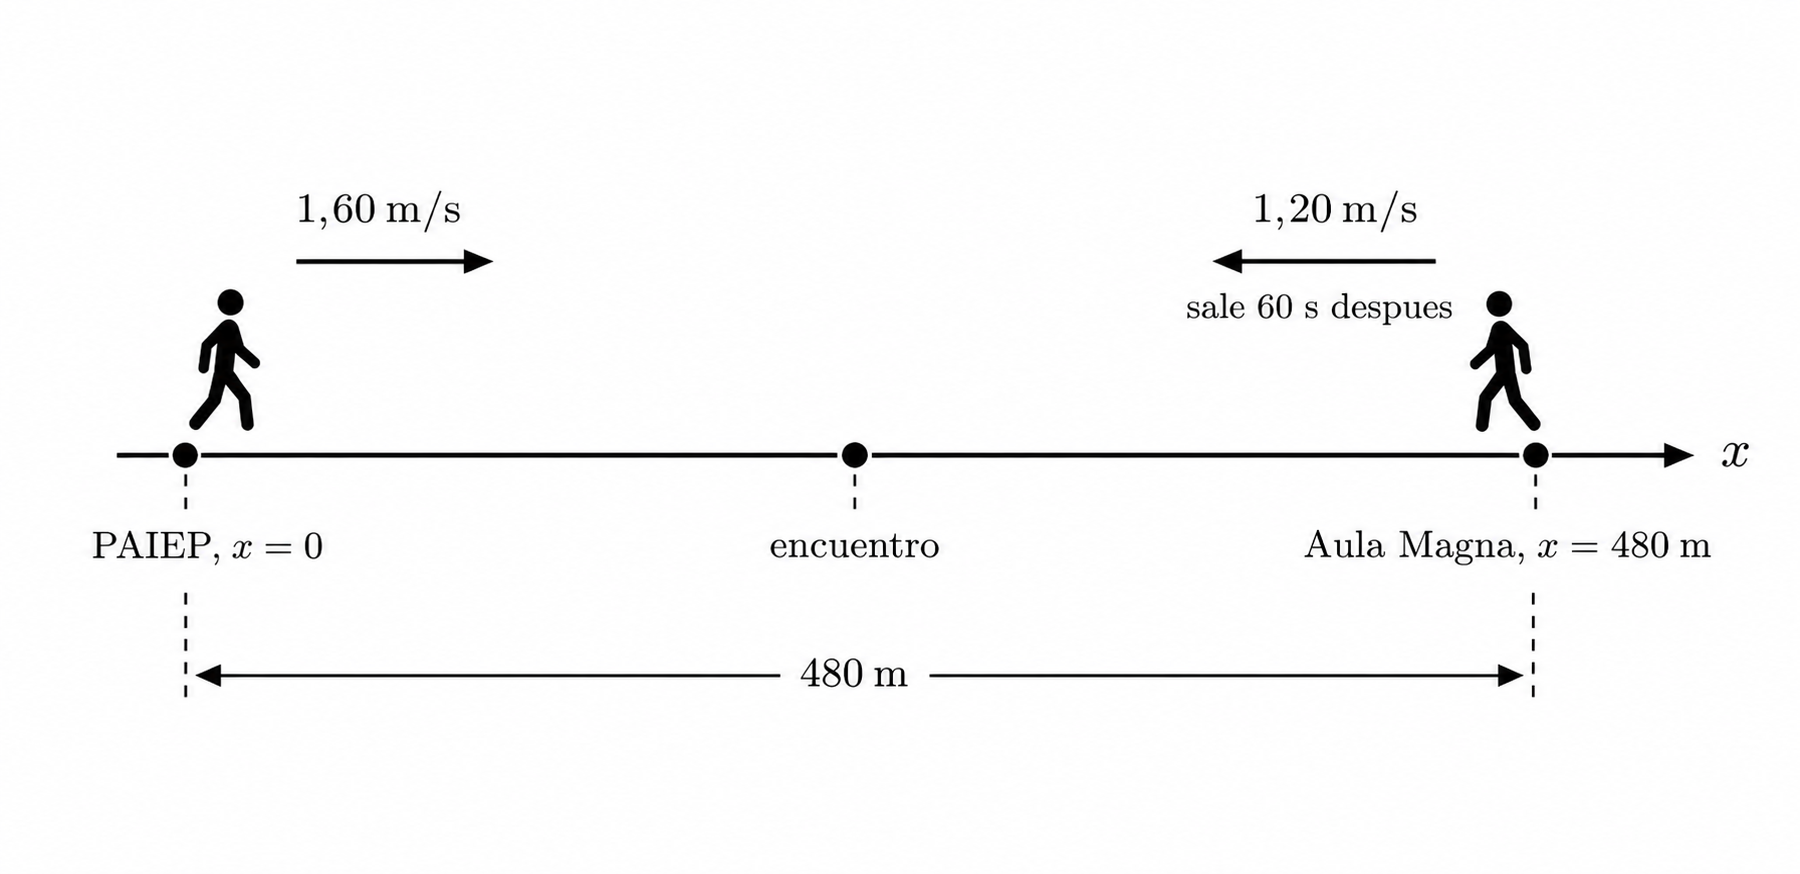
\includegraphics[width=0.86\textwidth]{./images/ejercicio2_mru.png}
\end{center}

\item \textbf{Gráfico de una ayudantía.} La posición de un pendón móvil usado para ordenar una fila de cachorros se modela por $x(t)=120+2{,}5t$, donde $x$ está en metros y $t$ en segundos.
\begin{enumerate}[label=\alph*)]
    \item Identifica la posición inicial.
    \item Identifica la velocidad.
    \item Determina el tiempo en que el pendón llega a $x=620\,\mathrm{m}$.
    \item Determina la posición para $t=90\,\mathrm{s}$.
\end{enumerate}
\begin{center}
    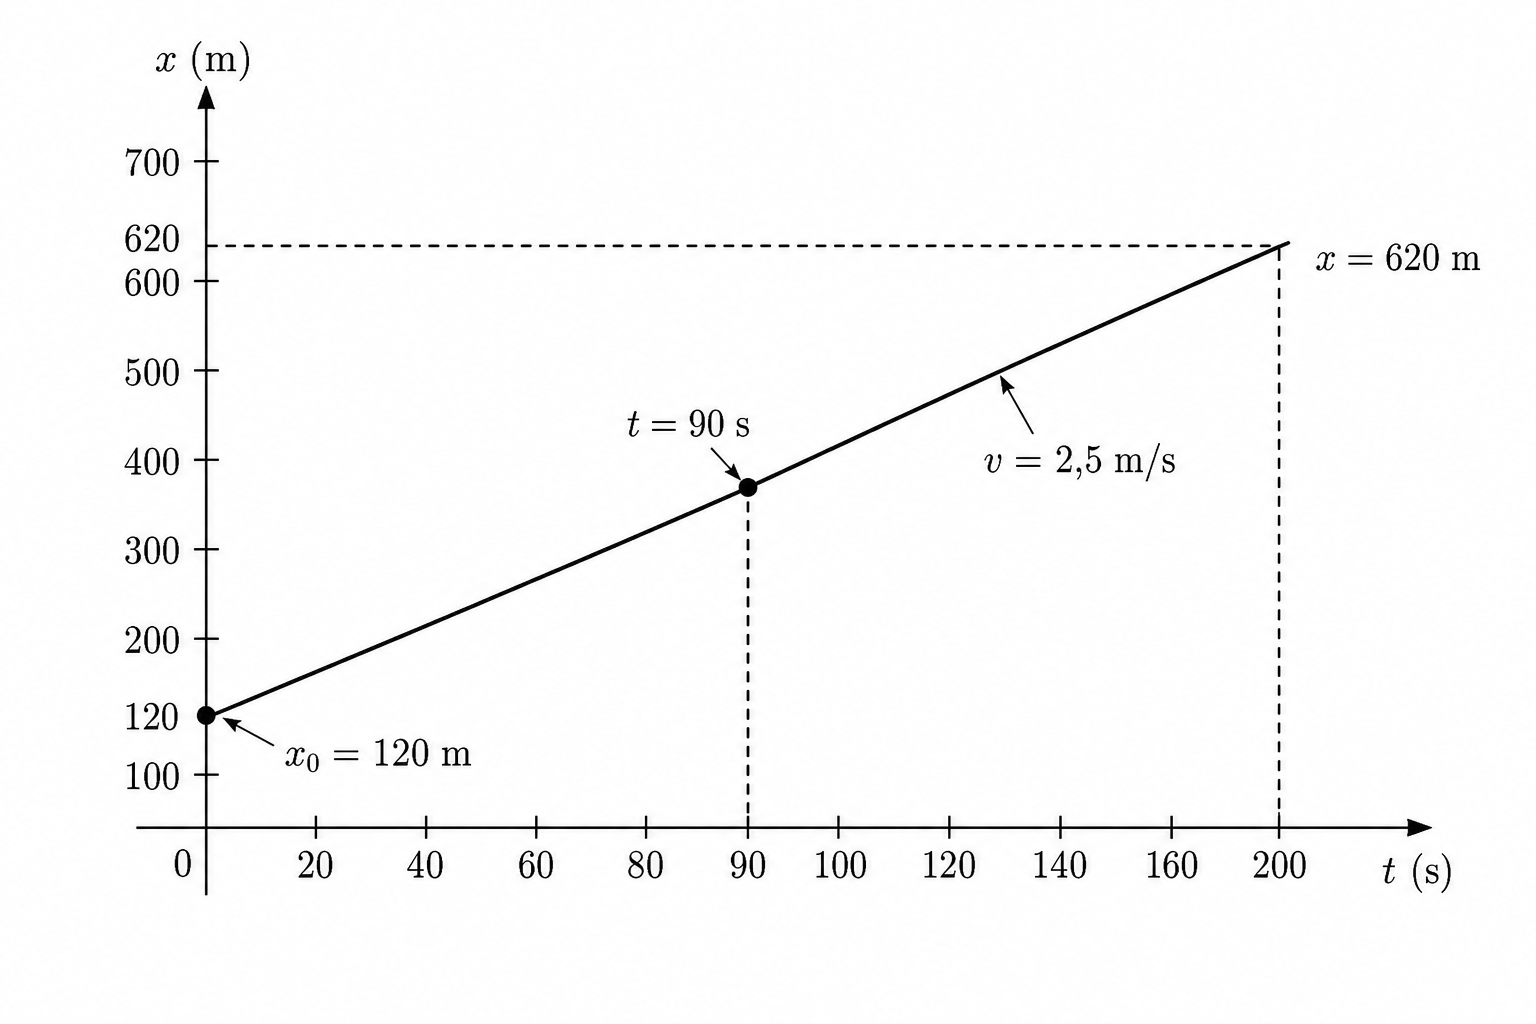
\includegraphics[width=0.86\textwidth]{./images/ejercicio3_mru.png}
\end{center}

\item \textbf{Pasillo con cinta transportadora.} Una cinta horizontal se mueve a $0{,}80\,\mathrm{m/s}$ hacia la derecha. Una estudiante camina sobre ella a $1{,}40\,\mathrm{m/s}$ respecto de la cinta.
\begin{enumerate}[label=\alph*)]
    \item Determina la rapidez respecto del suelo si camina en el mismo sentido de la cinta.
    \item Determina la rapidez respecto del suelo si camina en sentido contrario, pero todavía avanza hacia la derecha respecto del suelo.
    \item Si el tramo mide $132\,\mathrm{m}$, determina el tiempo en el caso del inciso a).
    \item Para el mismo tramo, determina el tiempo en el caso del inciso b).
\end{enumerate}
\begin{center}
    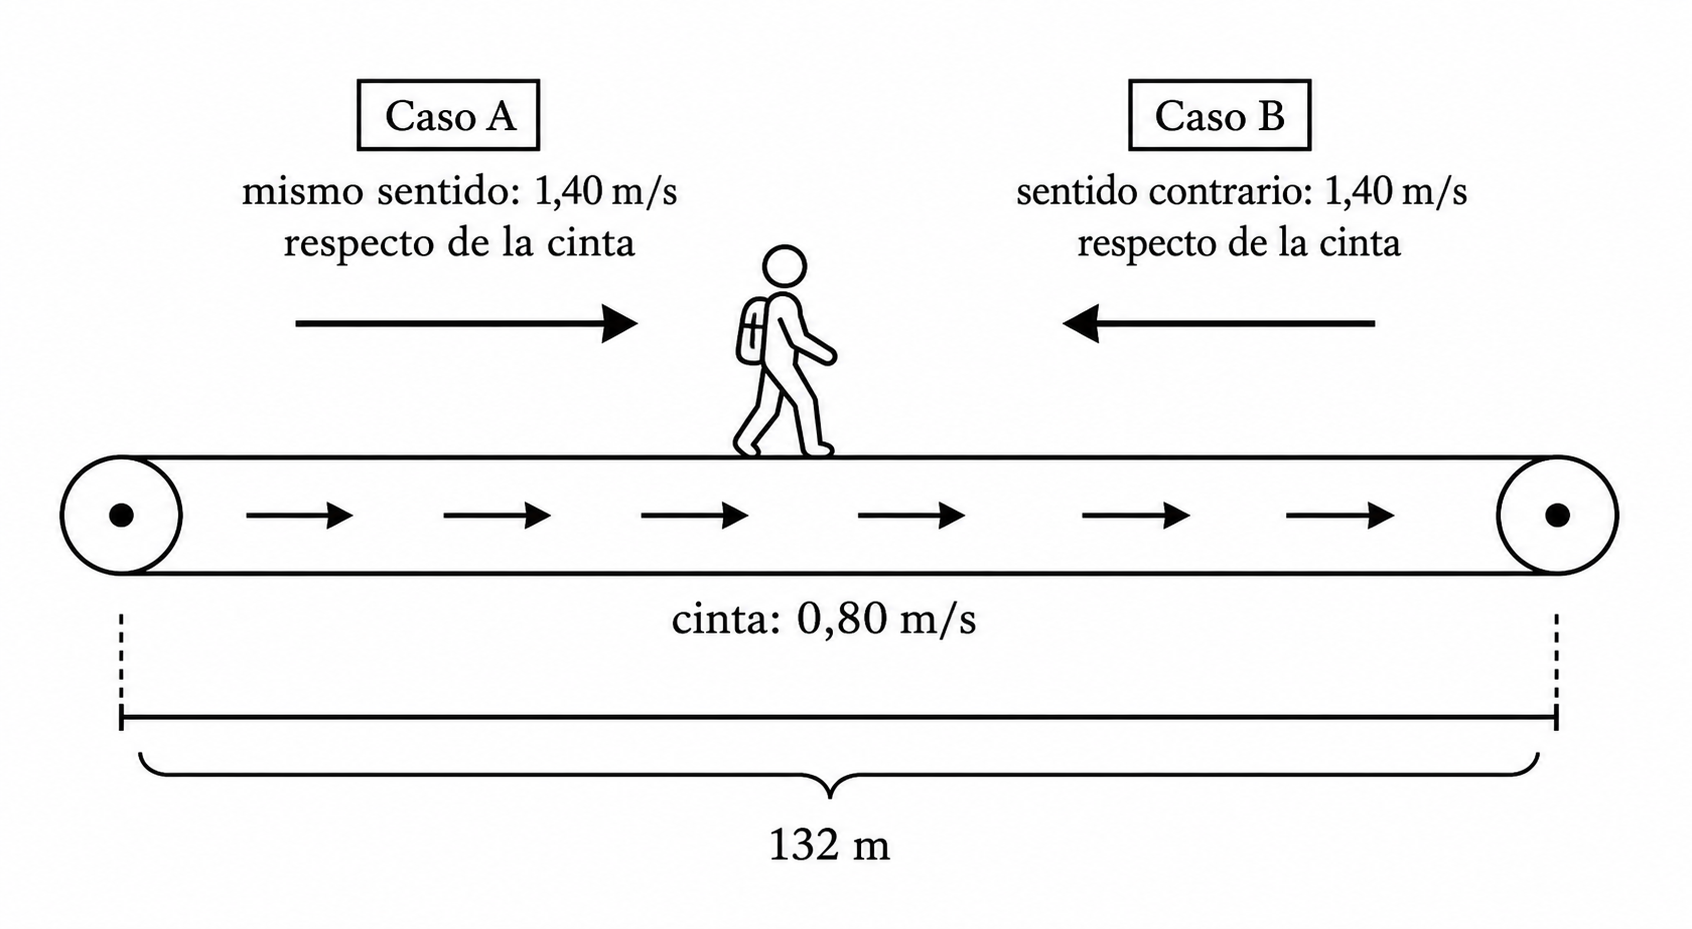
\includegraphics[width=0.86\textwidth]{./images/ejercicio4_mru.png}
\end{center}

\item \textbf{Mensaje imprudente en Alameda.} Un auto circula con rapidez constante de $72\,\mathrm{km/h}$. Cuando está en la posición $x=14{,}40\,\mathrm{km}$, el conductor mira un mensaje durante $6\,\mathrm{s}$. Un pórtico de seguridad del campus está en $x=14{,}50\,\mathrm{km}$.
\begin{enumerate}[label=\alph*)]
    \item Determina la distancia que recorre durante los $6\,\mathrm{s}$.
    \item Determina en qué instante, medido desde que mira el mensaje, pasa por el pórtico.
    \item Decide si el pórtico alcanza a registrar la conducta imprudente.
\end{enumerate}
\begin{center}
    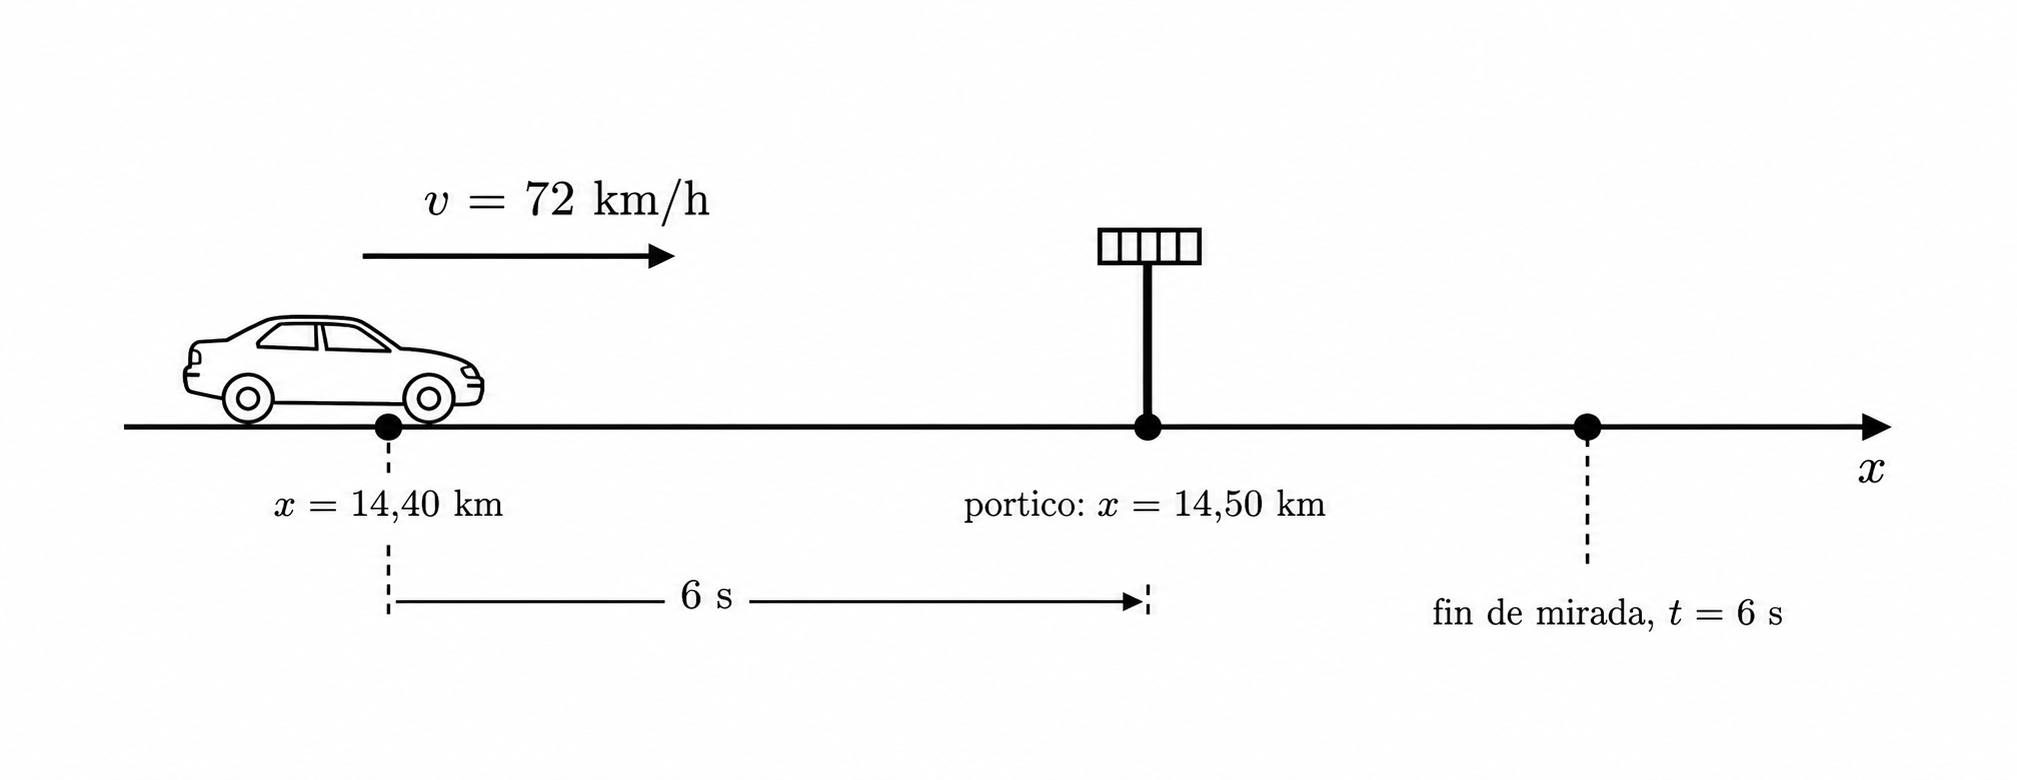
\includegraphics[width=0.86\textwidth]{./images/ejercicio5_mru.png}
\end{center}

\item \textbf{Fila de TNE.} Una cachorra avanza en una fila recta de $36\,\mathrm{m}$ hacia el punto de atención, con rapidez constante $0{,}18\,\mathrm{m/s}$. Una amiga parte desde el mismo inicio $45\,\mathrm{s}$ después y avanza con rapidez constante $0{,}30\,\mathrm{m/s}$.
\begin{enumerate}[label=\alph*)]
    \item Determina cuándo la amiga alcanza a la primera estudiante, medido desde que parte la primera.
    \item Determina la posición del alcance desde el inicio de la fila.
    \item Determina cuánto falta para llegar al punto de atención.
\end{enumerate}
\begin{center}
    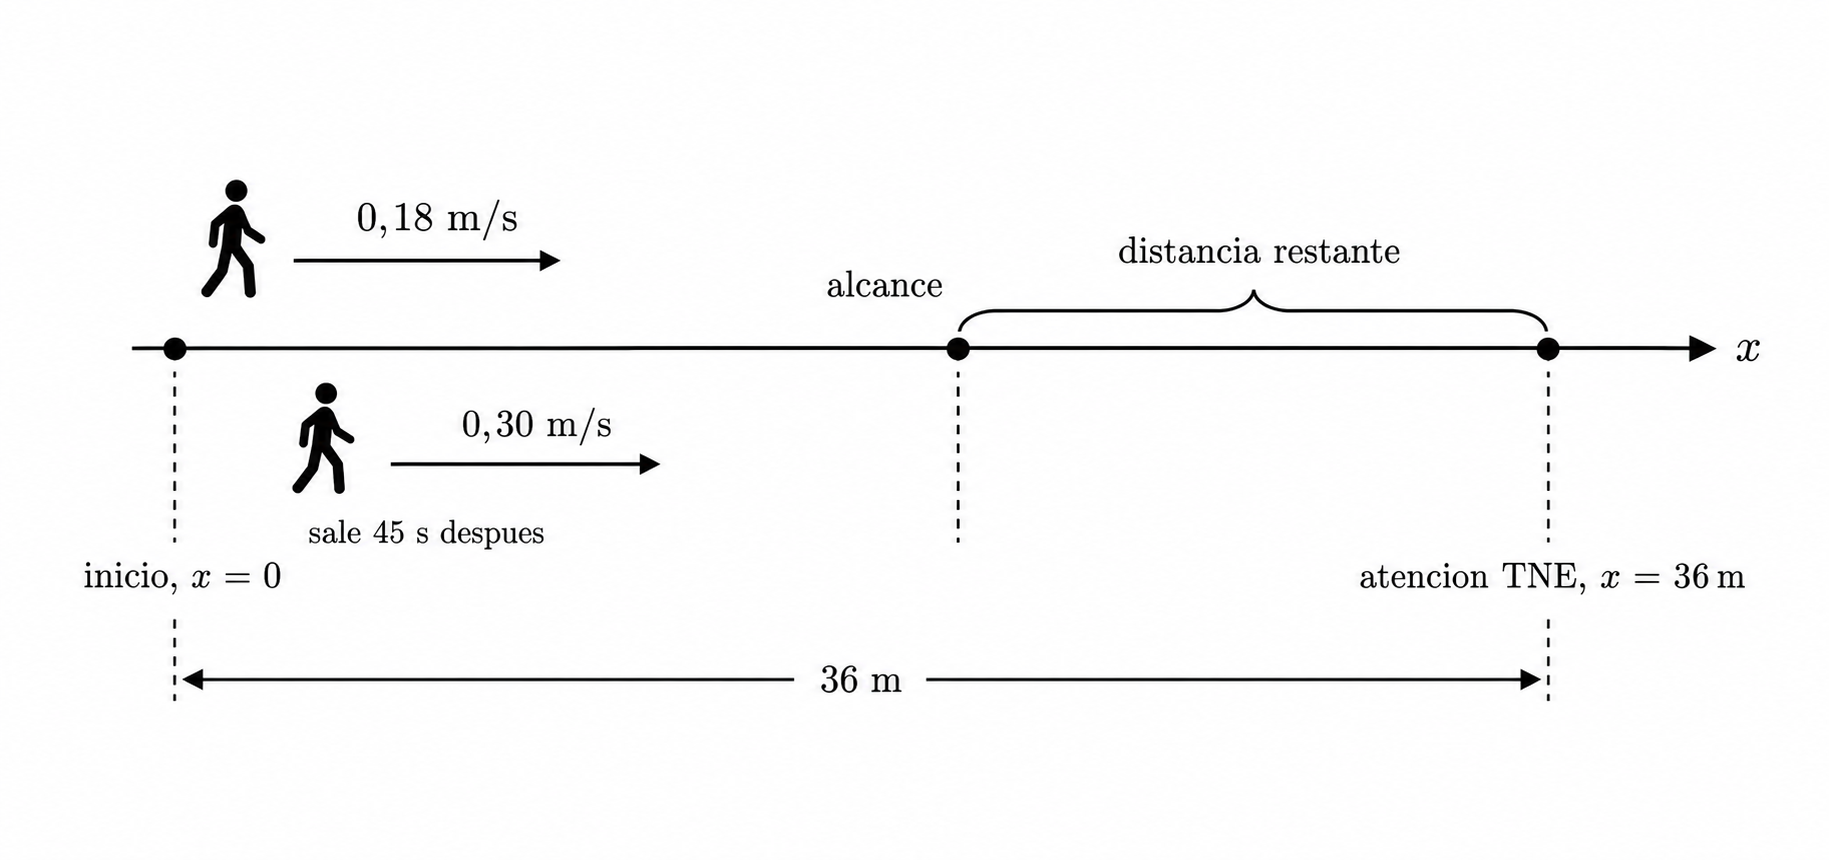
\includegraphics[width=0.86\textwidth]{./images/ejercicio6_mru.png}
\end{center}

\item \textbf{Reparto de guías.} Una ayudante camina desde la FING, $x=0$, con rapidez constante $1{,}50\,\mathrm{m/s}$. Al mismo tiempo, un ciclista parte desde el Planetario, a $1{,}800\,\mathrm{m}$ de distancia, con rapidez constante $5{,}00\,\mathrm{m/s}$ hacia la FING.
\begin{enumerate}[label=\alph*)]
    \item Determina el instante en que se encuentran.
    \item Determina la posición de encuentro medida desde la FING.
\end{enumerate}
\begin{center}
    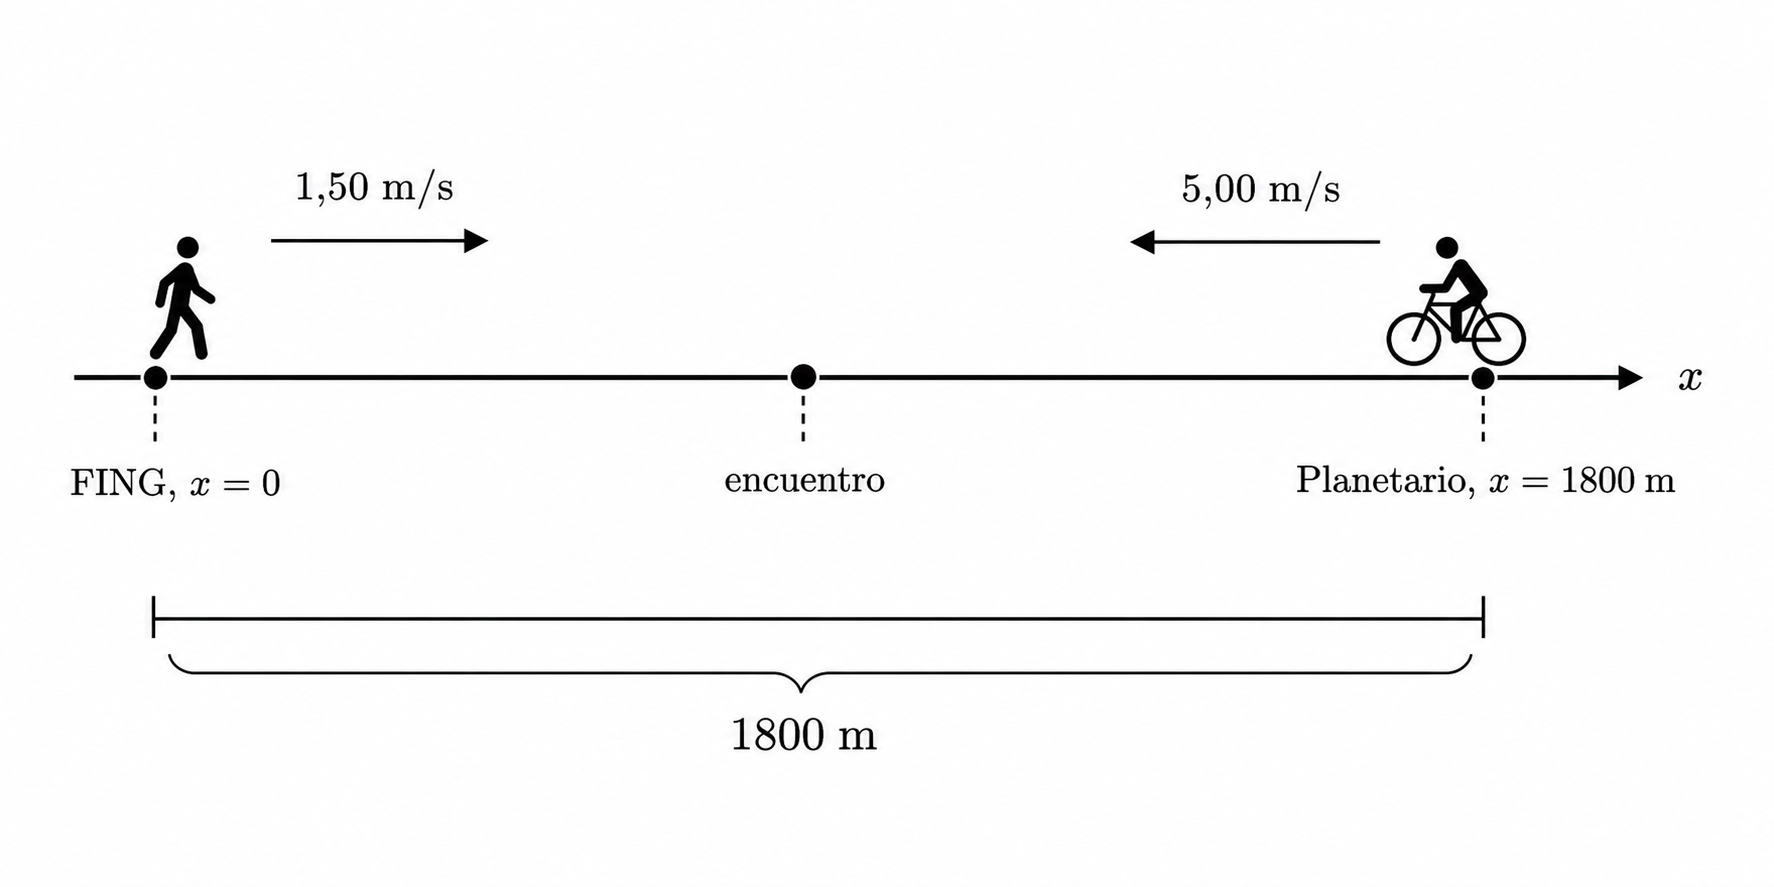
\includegraphics[width=0.86\textwidth]{./images/ejercicio7_mru.png}
\end{center}

\item \textbf{Tabla de posición de un pendón.} Durante una feria de bienvenida, se registra la posición de un pendón de Usach Premium sobre una línea recta:
\[
\begin{array}{c|ccc}
t\,(\mathrm{s}) & 0 & 20 & 50\\ \hline
x\,(\mathrm{m}) & 30 & 90 & 180
\end{array}
\]
\begin{enumerate}[label=\alph*)]
    \item Verifica si el movimiento es compatible con MRU.
    \item Determina la velocidad.
    \item Determina la posición para $t=75\,\mathrm{s}$.
    \item Determina el instante en que llega a $x=300\,\mathrm{m}$.
\end{enumerate}
\begin{center}
    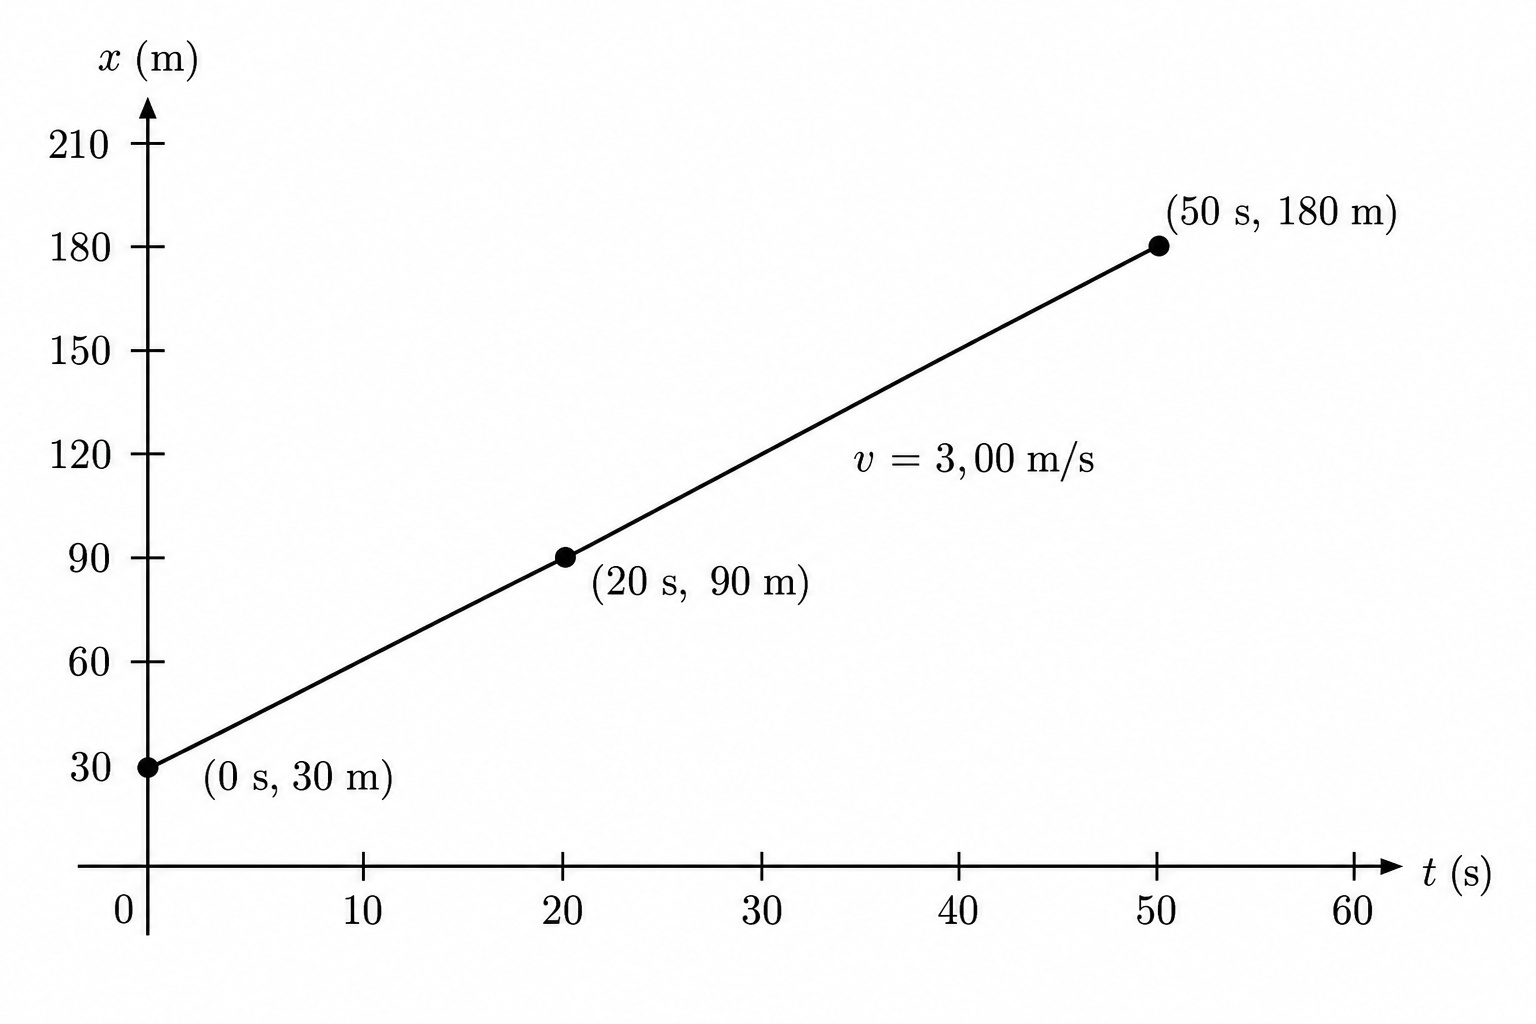
\includegraphics[width=0.86\textwidth]{./images/ejercicio8_mru.png}
\end{center}
\end{enumerate}

\vspace{0.5cm}
\begin{desafiobox}{DESAFÍO: Ruta Premium por el campus}
\small
El equipo de Usach Premium debe mover una caja de guías por tres tramos rectos consecutivos antes de una ayudantía masiva. En cada tramo el movimiento es rectilíneo uniforme:
\begin{itemize}[leftmargin=*]
    \item Tramo AB: $420\,\mathrm{m}$ a $1{,}40\,\mathrm{m/s}$.
    \item Tramo BC: $300\,\mathrm{m}$ a $2{,}00\,\mathrm{m/s}$.
    \item Tramo CD: $180\,\mathrm{m}$ a $1{,}20\,\mathrm{m/s}$.
\end{itemize}
\textbf{Pregunta:} Determina el tiempo total de traslado, la distancia total recorrida y la rapidez media de toda la ruta.
\begin{center}
    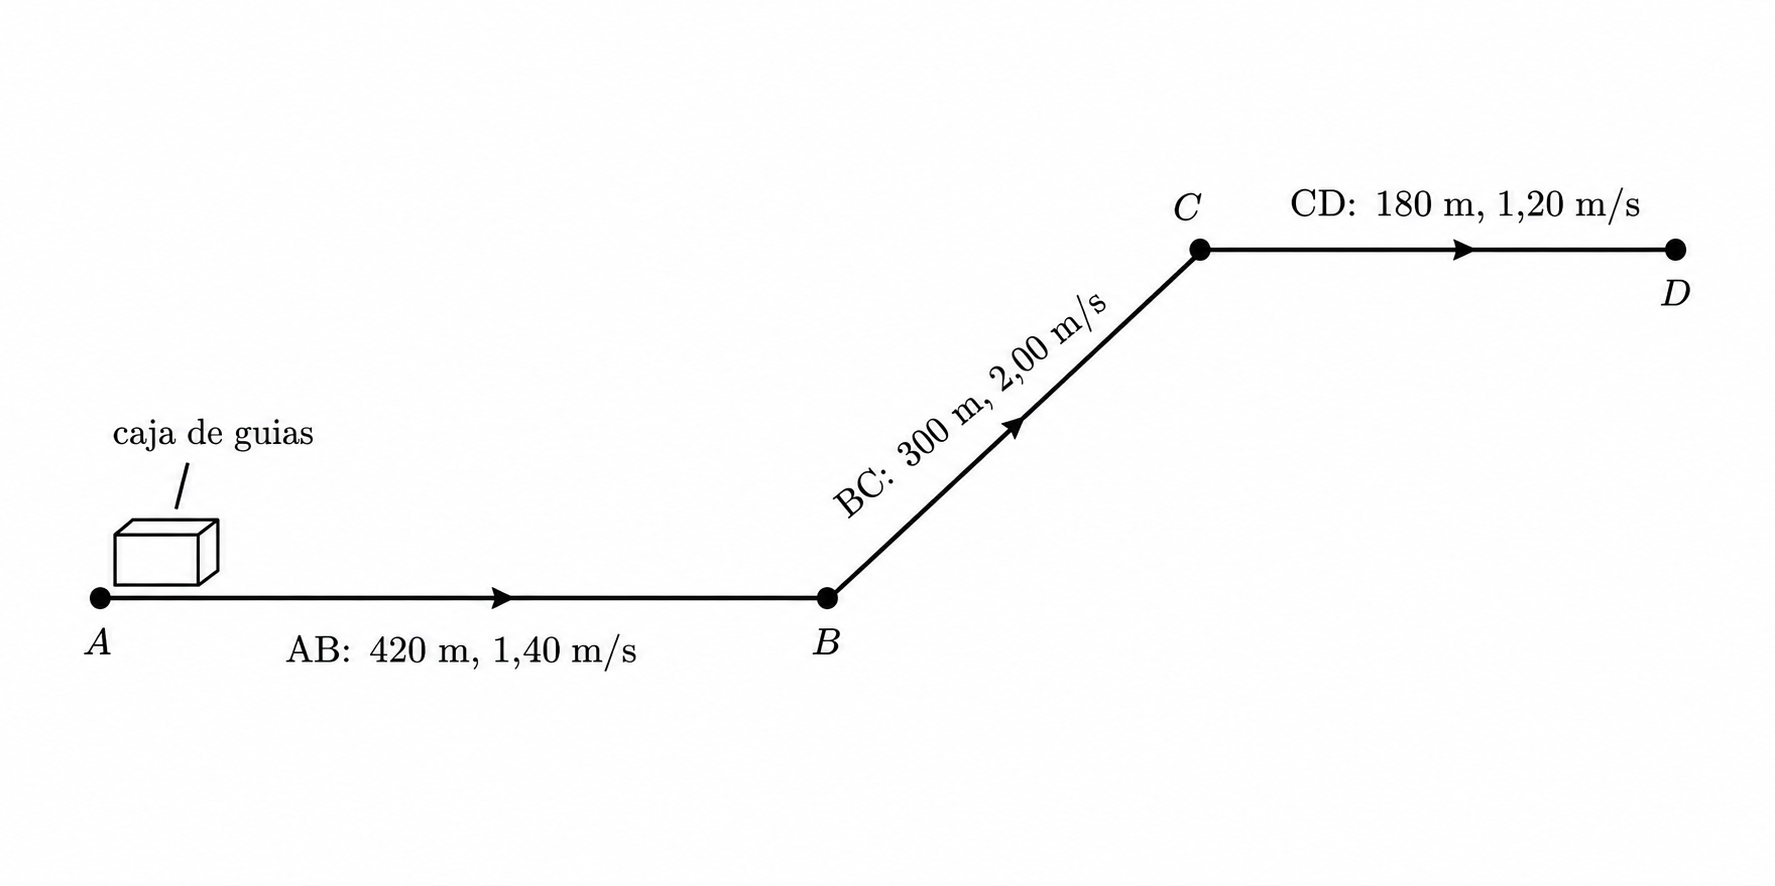
\includegraphics[width=0.86\textwidth]{./images/ejercicio9_mru.png}
\end{center}
\hrule\vspace{2mm}
\centering\footnotesize\textbf{Nota del Staff:} Si el resultado no está en SI, todavía no está listo para la pauta.
\end{desafiobox}
\end{ejercicios}

\begin{soluciones}
\begin{solbox}{I. Soluciones --- MRU básico y encuentros}
\begin{enumerate}[label=\color{azulFuerte}\bfseries\arabic*., leftmargin=*, itemsep=0.25cm]
    \item a) $80{,}00\,\mathrm{s}$ \quad b) $525{,}00\,\mathrm{m}$.
    \item a) $197{,}14\,\mathrm{s}$ \quad b) $315{,}43\,\mathrm{m}$ desde PAIEP.
    \item a) $x_0=120{,}00\,\mathrm{m}$ \quad b) $v=2{,}50\,\mathrm{m/s}$ \quad c) $200{,}00\,\mathrm{s}$ \quad d) $345{,}00\,\mathrm{m}$.
    \item a) $2{,}20\,\mathrm{m/s}$ \quad b) $0{,}60\,\mathrm{m/s}$ \quad c) $60{,}00\,\mathrm{s}$ \quad d) $220{,}00\,\mathrm{s}$.
\end{enumerate}
\end{solbox}
\begin{solbox}{II. Soluciones --- Aplicaciones tipo evaluación}
\begin{enumerate}[label=\color{azulFuerte}\bfseries\arabic*., leftmargin=*, itemsep=0.25cm, start=5]
    \item a) $120{,}00\,\mathrm{m}$ \quad b) $5{,}00\,\mathrm{s}$ \quad c) Sí, pasa por el pórtico durante el intervalo de distracción.
    \item a) $112{,}50\,\mathrm{s}$ \quad b) $20{,}25\,\mathrm{m}$ \quad c) $15{,}75\,\mathrm{m}$.
    \item a) $276{,}92\,\mathrm{s}$ \quad b) $415{,}38\,\mathrm{m}$ desde la FING.
    \item a) Sí, es compatible con MRU \quad b) $3{,}00\,\mathrm{m/s}$ \quad c) $255{,}00\,\mathrm{m}$ \quad d) $90{,}00\,\mathrm{s}$.
\end{enumerate}
\end{solbox}
\begin{solbox}{III. Solución --- Desafío}
\begin{enumerate}[label=\color{azulFuerte}\bfseries\arabic*., leftmargin=*, itemsep=0.25cm, start=9]
    \item Tiempo total: $600{,}00\,\mathrm{s}$; distancia total: $900{,}00\,\mathrm{m}$; rapidez media: $1{,}50\,\mathrm{m/s}$.
\end{enumerate}
\end{solbox}
\vspace{0.8cm}
\begin{center}\small\textbf{Usach Premium} --- ¡Nos vemos en la ayudantía!\\\textit{"Por y para estudiantes."}\end{center}
\end{soluciones}
\end{document}
